% Long rectangle [0,1]x[0,3]; curve y=3x^2 from (0,0) to (1,3); shade = rectangle minus under-curve.
% Shade boundary: (0,0)-(1,0)-(1,3)-curve reversed-cycle. Curve tip extends slightly above y=3.
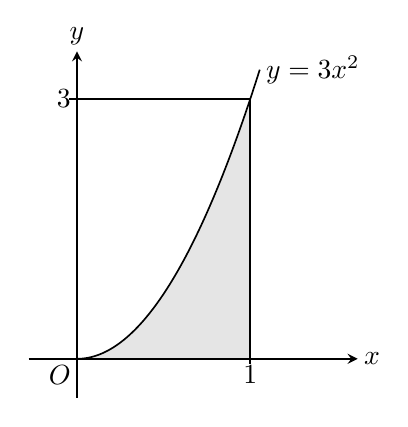
\begin{tikzpicture}[x=2.2cm,y=1.1cm,line width=.6pt,>=stealth]
\fill[gray!20] (0,0) -- (1,0) -- (1,3) -- plot[domain=1:0,samples=60] (\x,{3*\x*\x}) -- cycle;
\draw[->] (-0.28,0) -- (1.62,0) node[right,inner sep=0pt,xshift=2pt] {$x$};
\draw[->] (0,-0.45) -- (0,3.55) node[above,inner sep=0pt,yshift=2pt] {$y$};
\draw (0,3) -- (1,3);
\draw (1,0) -- (1,3);
\draw (1,0) -- (1,-0.06);
\node[below,inner sep=0pt,yshift=-2pt] at (1,0) {$1$};
\draw (-0.045,3) -- (0,3);
\node[left,inner sep=0pt,xshift=-2pt] at (0,3) {$3$};
\node[below left,inner sep=0pt,xshift=-2pt,yshift=-2pt] at (0,0) {$O$};
\draw[domain=0:1.055,samples=80] plot (\x,{3*\x*\x});
\node[right,inner sep=0pt,xshift=2pt] at (1.055,3.34) {$y=3x^2$};
\end{tikzpicture}
